\documentclass[12pt]{report}

\usepackage[a4paper, total={17cm, 24cm}]{geometry}
\usepackage{exercise}
\usepackage{amsmath}
\usepackage{tikz}

\renewcommand{\ExerciseHeader}{\noindent\textbf{\large\ExerciseName\ %
\ExerciseHeaderNB\ExerciseHeaderTitle
\ExerciseHeaderOrigin\medskip}}
\setlength{\QuestionIndent}{1.5em}

\newcommand{\answerbox}[2]{\hfill\break\\
        \framebox[\linewidth]{\parbox[c][#1][c]{\dimexpr\linewidth-2\fboxsep-2\fboxrule}{#2}}
}

\renewcommand{\arraystretch}{1.2} % vertical padding for tabular environment

\begin{document}

\hfill
\begingroup
\Large
\begin{tabular}{|l|p{6cm}|}
    \hline
    First \& last name &
    % YOUR NAME HERE
    \\ \hline
    NOMA UCLouvain & 
    % YOUR NOMA HERE
    \\ \hline
\end{tabular}
\endgroup
\vspace{1.5cm}

\noindent
\begingroup
    \Large
    \textbf{LINFO2266: Advanced Algorithms for Optimization}\\\\
    Project 4: Local Search
\endgroup
\vspace{0.2cm}

\begin{Exercise}[title={2Opt Move}]

Below is an instance of the Travelling Salesman Problem with 5 cities and a starting solution.

\begin{minipage}{0.5\textwidth}
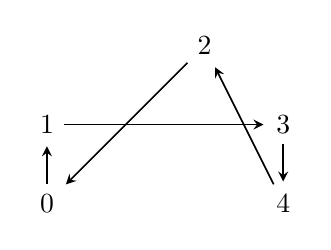
\begin{tikzpicture}[
            > = stealth, % arrow head style
            shorten > = 1pt, % don't touch arrow head to node
            auto,
            node distance = 3cm, % distance between nodes
            semithick % line style
        ]

        \tikzstyle{every state}=[
            draw = black,
            thick,
            fill = white,
            minimum size = 4mm
        ]
    % Define the nodes and their positions
    \node (0) at (0, 0) {0};
    \node (1) at (0, 1) {1};
    \node (2) at (2, 2) {2};
    \node (3) at (3, 1) {3};
    \node (4) at (3, 0) {4};
    
    % Draw edges between nodes
    \path[->] (1) edge node {} (3);
    \path[->] (3) edge node {} (4);
    \path[->] (4) edge node {} (2);
    \path[->] (2) edge node {} (0);
    \path[->] (0) edge node {} (1);
\end{tikzpicture}
\end{minipage}
\hfill
\begin{minipage}{0.4\textwidth}
\begin{tabular}{c|cc}
 City ID & X position & Y position \\ \hline
 0 & 0 & 0 \\
 1 & 0 & 10 \\
 2 & 20 & 20 \\
 3 & 30 & 10 \\
 4 & 30 & 0
\end{tabular}
\end{minipage}\\\\\

\Question This is the initial circuit representation [0,1,2,3,4]. Apply an imroving 2Opt move of your choice. Show the sequence of the circuit after and give the delta cost on the objective (it should be negative number).
\answerbox{6cm}{
% YOUR ANSWER HERE
}

\end{Exercise}

\newpage


\begin{Exercise}[title={Initialization}]


\Question Your PilotInitialization class extends the BeamSearchInitialization class. Explain how you achieved this design (how does it avoid code duplication?).
\answerbox{10cm}{
% YOUR ANSWER HERE
}

\Question Justify the time complexity of your implementation.
\answerbox{10cm}{
% YOUR ANSWER HERE
}

\end{Exercise}

\newpage

\begin{Exercise}[title={Improving the solution}]

\Question Using RandomInitialization, compare Tabu Selection with Best Selection by plotting the objective function of the current candidate at each iteration over 200 iterations on the instance data/TSP/gr48.xml. Overlay the curves for tabu lengths of 3 and 15.
\answerbox{6cm}{
% YOUR ANSWER HERE
}

\Question Using a local search with random initialization and BestSelection within a 2Opt neighborhood as a baseline, implement an enhanced local search incorporating any components of your choice (e.g., selection, initialization, meta-heuristics). Explain your choices, and compare both approaches by showing the progression of the best solution found over the iterations for each method. Since the process may involve pseudorandom number generators, it is good practice to represent the standard deviation around these curves.

\answerbox{10cm}{
% YOUR ANSWER HERE
}

\end{Exercise}

\end{document}